\section{Introduction}

A robot that can put a bottle on a stove should be able to interpret placing it to the right of that stove as a new combination of familiar concepts.
It should also be able to combine this behavior with placing a bowl and moving a package of cheese, without requiring demonstrations of every complete sequence.
These capabilities involve composition at 2 levels: within a subtask, where entities, actions, and modifiers determine the desired interaction, and between subtasks, where individual behaviors must execute in order from the states left by preceding actions.

Imitation learning has made substantial progress through action chunking~\cite{zhao2023act}, generative action prediction~\cite{chi2023dp}, and large-scale vision-language-action pretraining~\cite{physicalintelligence2025pi05}.
Point-based policies further provide geometric representations for observations and actions~\cite{ze2024dp3,haldar2025pp,haldar2026pb}.
However, geometry alone does not specify what an entity should do in a task.
The same scene may require different motions depending on the instructed action or relation, and success on individual tasks does not establish that a policy can compose them into longer instructions.
This motivates an explicit interface between task semantics, entity geometry, and action generation.

We introduce GraphPoint, which represents an active subtask as a graph of actor, patient, and target point entities.
These roles identify the gripper, the manipulated object, and the reference entity, respectively.
A shared encoder processes each entity locally and exchanges temporal summaries through an actor--patient--target chain.
Role embeddings condition local geometry encoding, while separately encoded action types and modifiers condition interaction and trajectory decoding.
The policy predicts future actor points in the same tool center point (TCP)-relative space as its observations, and geometric alignment converts these predictions into robot poses.
Role-aware point collapse augments object geometry during training, and a progress head supports reuse of the policy across subtasks.
Fig.~\ref{fig:representation_comparison} contrasts this interface with image-, scene-point-, and entity-point-based policies.

\begin{figure}[t]
\centering
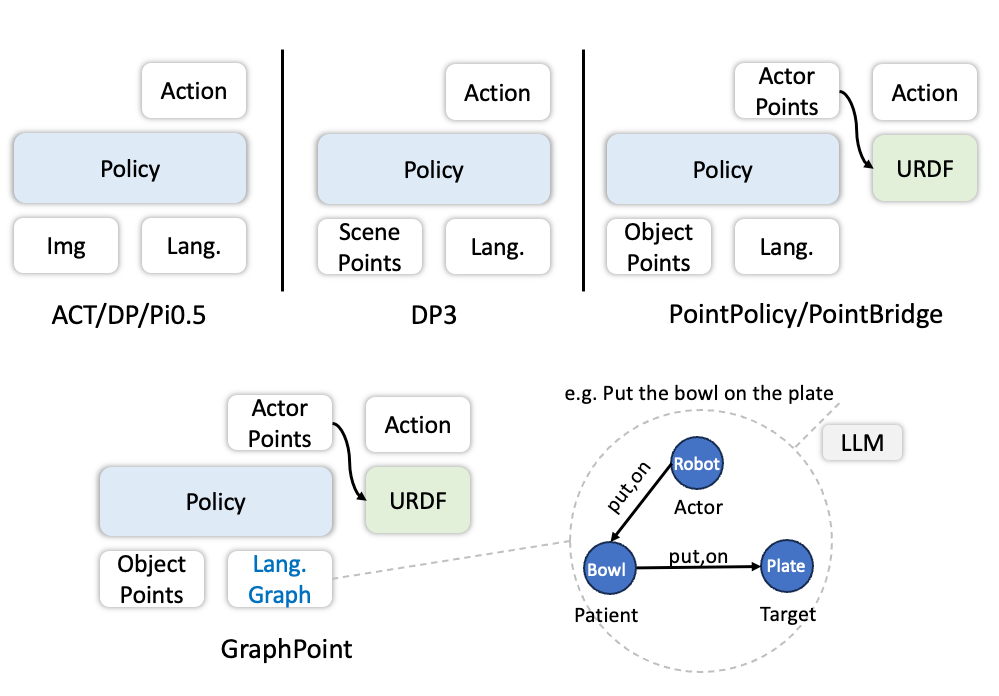
\includegraphics[width=\columnwidth]{fig/compare.png}
\caption{Policy representation interfaces.
GraphPoint organizes entity points into a language-conditioned role graph and converts predicted actor points into robot actions through gripper geometry.}
\label{fig:representation_comparison}
\end{figure}

To isolate these capabilities, we introduce CoMani, a LIBERO-based benchmark~\cite{liu2023libero} with suites for modifier, action-type, and sequential composition.
Matched initial scenes reduce visual task shortcuts, and atomic-only training separates skill acquisition from sequence execution.
Our contributions are:
\begin{itemize}
    \item CoMani, a benchmark addressing the need to distinguish composition of modifiers, action types, and atomic skills through controlled in-distribution (ID) and out-of-distribution (OOD) splits over 18 modifier tasks, 10 action tasks, and 6 sequences.
    \item GraphPoint, a framework coupling semantic entity graphs with task-conditioned point-trajectory control and progress-based subtask switching, validated through baseline comparisons and component ablations on CoMani.
\end{itemize}
